\documentclass[11pt, a4paper]{article}
\usepackage[utf8]{inputenc}
\usepackage[margin=.7in]{geometry}
\usepackage{listings}
\usepackage{setspace}
\usepackage{xcolor}
\usepackage{titlesec}
\usepackage{enumitem}
\usepackage{amssymb}
\usepackage{amsmath}
\usepackage{bm}
\usepackage{multicol}
\usepackage{graphicx}
\graphicspath{{./Figures/}}
\usepackage{color}
\usepackage{hyperref}
\hypersetup{
	colorlinks=true,
	linkcolor=blue,
	urlcolor=blue,
}
\titleformat*{\section}{\LARGE\bfseries\filcenter}
\titleformat*{\subsection}{\Large\bfseries}
\titleformat*{\subsubsection}{\large\bfseries}
\definecolor{codegreen}{rgb}{0,0.5,0}
\definecolor{codegray}{rgb}{0.5,0.5,0.5}
\definecolor{codered}{rgb}{0.78,0,0}
\definecolor{codepurple}{rgb}{0.58,0,0.68}
\definecolor{backcolour}{rgb}{0.95,0.95,0.92}
\lstdefinestyle{Pythonstyle}{
	language = Python,
    backgroundcolor=\color{backcolour},   
    commentstyle=\color{gray},
    keywordstyle=\color{codegreen},
    numberstyle=\tiny\color{codegray},
    stringstyle=\color{codered},
    basicstyle=\ttfamily\footnotesize,
    breakatwhitespace=false,         
    breaklines=true,                 
    captionpos=b,                    
    keepspaces=true,                 
    numbers=left,                    
    numbersep=5pt,                  
    showspaces=false,                
    showstringspaces=false,
    showtabs=false,                  
    tabsize=2,
    morekeywords = {as},
    keywordstyle = \color{codegreen}
}
\lstset{style=Pythonstyle}

\begin{document}
	\begin{titlepage}
		\begin{center} \Huge \textbf{Deep Learning in Python} \end{center}
		\tableofcontents
		\newpage
	\end{titlepage}
%%%% PAGE 1 %%%%

	\begin{spacing}{1.1}
	\section{Neural Networks and Deep Learning}
	\subsection{Logistic Regression as a Neural Network}
	\subsubsection{Introduction to Logistic Regression}
	\begin{minipage}[c]{10cm}
	A single \textbf{neural network} can be built off of an input (x), an activation layer known as a \textit{neuron}, and producing an output (y). A larger neural network is then formed by taking many of the single neurons and stacking them together. Each \textit{feature} ($x_1, x_2,..., x_n$) can be used as an input to the activation layers to produce our output y. For the below example, we say that the layer in the middle is \textit{densely connected} since every feature is in input.
	\end{minipage}
	\begin{minipage}[c]{4cm}
	\hspace*{6mm} 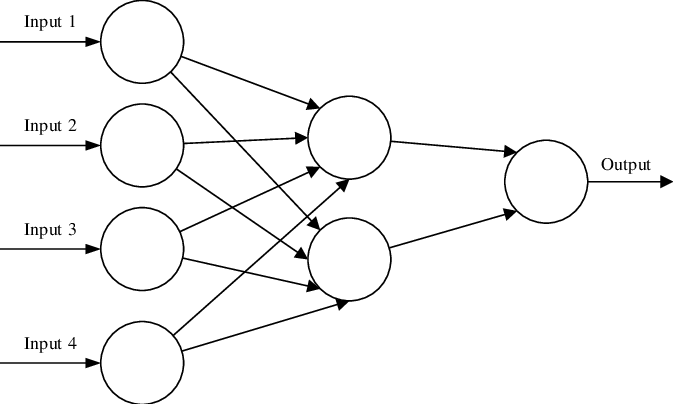
\includegraphics[scale=.25]{nn_intro} 
	\end{minipage} \vspace*{3mm} \\~\\
	To store an image, your computer stores three different matrices corresponding to the red, green, and blue channel (RGB values). So if your input image is 64x64 pixels, you will have three 64x64 matrices. To unroll these values into a \textbf{feature vector}, we will add values from all 3 vectors into a single x vector, where $n_x$ is the number of features in the vector (in this case, 12288). \vspace*{2mm} \\
	In \textbf{binary classification}, our goal is to learn a classifier that can input an image represented by feature vector \textit{x} and predict whether the corresponding label y is a 1 or 0 (1 for cat, 0 for non cat). \vspace*{2mm} \\
	Here is some common notation we will be using: \vspace*{1mm} \\
	\hspace*{3mm} - Single training example: (x,y) where $x \in \mathbb{R}^{n_x}$, y $\in \{0,1\} $ \vspace*{1mm} \\
	\hspace*{3mm} - M training examples: $\{(x^1, y^1), ..., (x^m, y^m)\}$  \vspace*{1mm} \\
	\hspace*{3mm} - Matrix X: $\begin{bmatrix} | & | & ... & | \\ x^1 & x^2 & ... & x^m \\ | & | & ... & | \end{bmatrix}$ where rows = $n_x$, columns = m. In Python, X.shape = ($n_x$, m). \vspace*{2mm} \\
	\hspace*{3mm} - Matrix Y: $\begin{bmatrix} y^1, y^2, ..., y^m \end{bmatrix}$ where Y.shape = (1, m) \\~\\
	Given x, we want an estimate known as $\hat{y}$ = P(y=1$|$x) given the following parameters: $x \in \mathbb{R}^{n_x}$, $w \in \mathbb{R}^{n_x}$, and $b \in \mathbb{R}$. We want out output to be $0 \leq \hat{y} \leq 1$, so we will use the \textbf{sigmoid function} to find our output, which will be: $$ \hat{y} = \sigma (z) \;\; \text{where}\;\; z = w^Tx + b \;\; \text{and}\;\; \sigma(z) = \frac{1}{1+e^{-z}}$$ If z is large, then $\sigma(z)$ will be very close to 1. But if z is a large negative number, then $\sigma(z)$ will be very close to 0. So given $\{(x^1, y^1),...,(x^m,y^m)\}$ we want $\hat{y}^i \approx y^i$
	\subsubsection{Logistic Regression Cost Function}
	We will associate $x^i$, $y^i$, and $z^i$ with the $i^{th}$ training example of our data. We will need to define a \textbf{loss function}, with respect to a single training example, to measure how good our output ($\hat{y}$) is when the true label is y. Since we are using gradient descent, we will define the following loss function: $$ \mathcal{L}(\hat{y},y) \; = \; -(y\,log(\hat{y}) \; + \; (1-y)\,log(1-\hat{y}))  $$ We want this loss function to be as small as possible. Lets look at the two cases: \vspace*{1mm} \\
	\hspace*{2mm} If y=1: $ \mathcal{L}(\hat{y},y) \, = \, -y\,log(\hat{y})$ and we want this to be as small as possible ($\hat{y}$ large). \\
	\hspace*{2mm} If y=0: $ \mathcal{L}(\hat{y},y) \, = \, -\,log(1-\hat{y})$ and we want this to be large ($\hat{y}$ small). \newpage
%%%% PAGE 2 %%%%

	\noindent To train the parameters \textit{w} and \textit{b}, we need to define a \textbf{cost function}, which measures how well your doing on an entire training set (cost of the parameters). We will define this as: \\ $$ J(w,b)\, = \, \frac{1}{m}\, \sum_{i=1}^{m}\, \mathcal{L}(\hat{y}^i,y^i) \; = \; -\frac{1}{m}\, \sum_{i=1}^{m}\, [(y^i\,log(\hat{y}^i) \; + \; (1-y^i)\,log(1-\hat{y}^i))] $$
	\subsubsection{Gradient Descent}
	\begin{minipage}[c]{10cm}
	We want to find the values of w and b that will \textit{minimize} the cost function J(w,b). Our cost function that we defined is convex (only one minimum). So we will initialize (w,b) to a random value, typically zero, and will take steps downhill in the steepest direction it can. Eventually it will converge to a minimum value and find our parameter values.
	\end{minipage}
	\begin{minipage}[c]{6cm}
	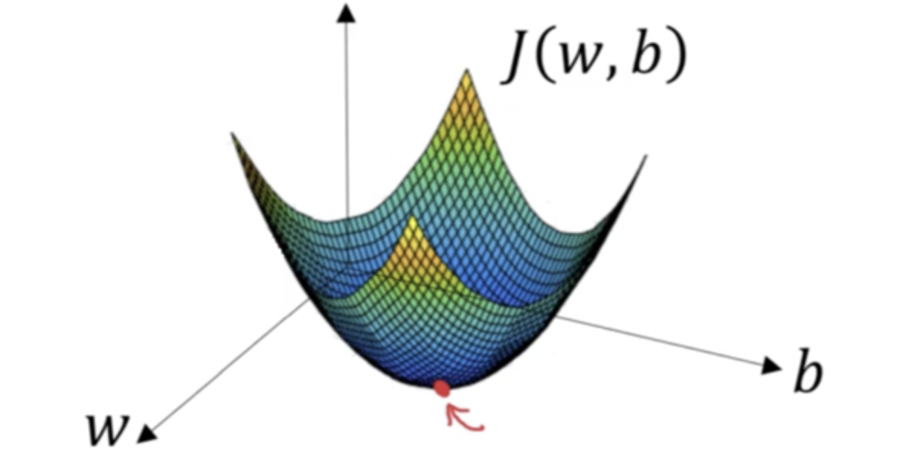
\includegraphics[scale=.4]{grad_desc}
	\end{minipage} \vspace*{4mm} \\~\\
	\textbf{Gradient descent} will repeatedly update the value of w and b with the formula: $$ w \, = \, w \, - \, \alpha \, \frac{ \partial J(w,b)}{\partial w} \; , \; b \, = \, b \, - \, \alpha \, \frac{\partial J(w,b)}{\partial b} $$ where $\alpha$ is our learning rate that we set multiplied by the partial derivative (since there are two variables) of the cost function with respect to the given parameter. \vspace*{2mm} \\
	We want to modify out \textit{w} and \textit{b} parameters in order to reduce the loss when performing gradient descent on our Logistic Regression. We can set up a computation graph to find the derivatives through \textbf{backpropagation}. We will do this for a \textit{single} training example, lets remind ourselves of our equations and the graph: \\
	\begin{minipage}[c]{8cm}
	$ z = w^Tx+ b$ \\
	$\hat{y} = a = \sigma(z)$ \\
	$\mathcal{L}(a,y) \; = \; -(y\,log(a) \; + \; (1-y)\,log(1-a))$ \\
	\end{minipage}
	\begin{minipage}[c]{6cm}
	\vspace*{2mm}
	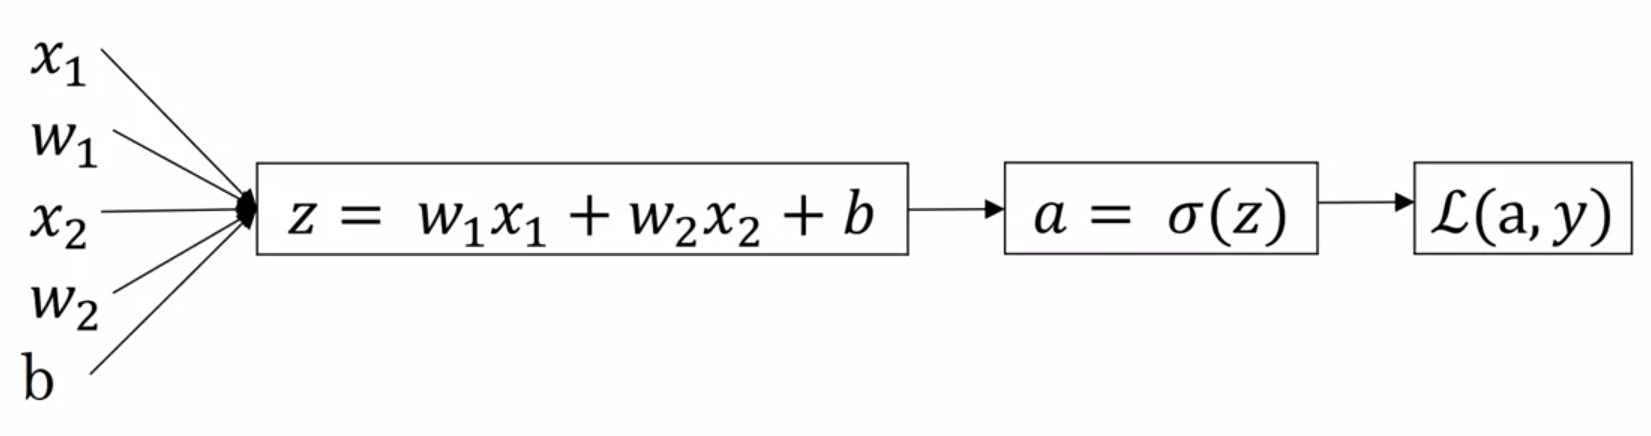
\includegraphics[scale=.2]{comp_graph}
	\end{minipage} \vspace*{1mm} \\~\\
	The first back step is to compute ``da'' = $\frac{\partial \mathcal{L}(a,y)}{\partial a}\; = \; \frac{-y}{a} - \frac{1-y}{1-a}$ \vspace*{2mm}\\
	Next we step back again and compute ``dz'' = $\frac{\partial \mathcal{L}(a,y)}{\partial z}\; = \; \frac{\partial \mathcal{L}}{\partial a}*\frac{\partial a}{\partial z}\; = \; a(1-a)*(\frac{-y}{a} + \frac{1-y}{1-a})\; = \; a-y$ \vspace*{2mm}\\
	The final step back is to find how much to change our $w_1$, $w_2$, and $b$ values. We can do this by: \vspace*{1mm} \\
	\hspace*{2mm} - Calculating: $\frac{\partial \mathcal{L}}{\partial w_1}\;$ = ``$dw_1$" = $x_1 * dz$, ``$dw_2$" = $x_2 * dz$, and ``$db$" = $dz$ \vspace*{1mm} \\
	\hspace*{2mm} - Then update our variables: $w_1 \; = \; w_1 - \alpha* dw_1$, $w_2 \; = \; w_2 - \alpha* dw_2$, and $b \; = \; b - \alpha* dz$ \\~\\
	Now we want to \textbf{perform gradient descent on m examples}. This will use the cost function (not the loss function like we did on a single example). We will write sudo-code for Python that implements this m example gradient descent (assume that $n_x$ = 2): \\
	\begin{minipage}[c]{8cm}
	Initialize: J=0, $dw_1$=0, $dw_2$=0, db=0 \\
	for i=1 to m: \\
	\hspace*{2mm} $z^i = w^Tx^i+b$\\
	\hspace*{2mm} $z^i = \sigma(z^i)$\\
	\hspace*{2mm} $J+= -[(y^i\,log(a^i) \; + \; (1-y^i)\,log(1-a^i))]$\\
	\hspace*{2mm} $dz^i = a^i - y^i$\\
	\hspace*{2mm} $dw_1 += x_1^i*dz^i$\\
	\hspace*{2mm} $dw_2 += x_2^i*dz^i$\\
	\hspace*{2mm} $db += dz^i$
	\end{minipage}
	\begin{minipage}[c]{8cm}
	\vspace*{2mm}
	After the loop, we then take the average and update our varaibles: \vspace*{1mm} \\
	J /= m \\
	$dw_1$ /= m \\
	$dw_2$ /= m \\
	db /= m \vspace*{1mm} \\
	$w_1 \; = \; w_1 - \alpha* dw_1$ \\
	$w_2 \; = \; w_2 - \alpha* dw_2$\\
	 $b \; = \; b - \alpha* db$
	\end{minipage} \newpage
%%%% PAGE 3 %%%%

	\subsection{Vectorization in Python}
	We often find ourselves training on big data sets and we need our code to run as fast as possible. This is where \textbf{vectorization} comes into play. One example is when we want to calculate $ z = w^Tx + b$. We can use \textit{np.dot(w, x) + b} in Python rather than a \textit{for loop} to decrease our run time by a significant amount. The takeaway from this section is that in deep learning, we want to avoid for loops and use vectorized code (such as NumPy methods) to save time when using large data sets. 
	\subsubsection{Vectorizing Logistic Regression}
	Remember previously we had defined a matrix, X = $\begin{bmatrix} | & | & ... & | \\ x^1 & x^2 & ... & x^m \\ | & | & ... & | \end{bmatrix}$, that contains the training data. \vspace*{1mm}\\ In order to vectorize finding $ z^i = w^Tx^i + b$ for m training examples, we can instead create a vector of these \textit{z} values, denoted by \textit{Z}.  $$ Z\; =\; [z^1,\; z^2,...,\; z^m] = w^TX + [b,\, b,\,...,\,b] = [w^tx^1+b,\; w^tx^2+b,\;...,\; w^tx^m+b]$$ 
	We will also want to vectorize our sigmoid function, which we will see in our programming assignment where we find A = [$a^1, a^2,..., a^m$] = $\sigma(z)$. These are the forward propogations. \\~\\
	Next we will want to vectorize the remaining steps in order to speed up our code. Lets begin with $dz^i = a^i - y^i$. Instead of looping through each training example, we can use vectors we already created, A = [$a^1, a^2,..., a^m$]  and Y = [$y^1, y^2,..., y^m$] . We can define: $$ dZ = A - Y = [a^1-y^1, a^2-y^2,..., a^m-y^m] = [dz^1, dz^2, ..., dz^m] $$ Now we want to vectorize dw for all training examples. We know that $dw^i += x^i_m*dz^i$ must be updated fo each example and then divided by the total number of examples (m), so we define this as: $$ dw = \frac{1}{m}\,X\, dz^T = \frac{1}{m}\, \begin{bmatrix} | & | & ... & | \\ x^1 & x^2 & ... & x^m \\ | & | & ... & | \end{bmatrix} \begin{bmatrix} dz^1\\ | \\ dz^m \end{bmatrix}  = \frac{1}{m}\, [x^1dz^1 + ... + x^m dz^m]$$ Finally, we see $db$ is the sum of $dz^i$ divided by the total number of examples (m), we can write this as: $$ db \, = \, \frac{1}{m} \sum_{i=1}^m dz^i = np.sum(dZ)$$
	Note that the below steps are only one step of gradient descent, you would still need a for loop to perform multiple steps. The new vectorized gradient descent can now be written as: \vspace*{2mm} \\
	$ Z = w^TX+b$ \\
	$ A = \sigma(z)$ \\
	$ dZ = A-Y$ \\
	$ dw = \frac{1}{m}\,X\,dz^t$ \\
	$ db = \frac{1}{m}\ np.sum(dZ)$ \\
	$w = w - \alpha dw$\\
	$b = b - \alpha db$ \newpage
%%%% PAGE 4 %%%%

	\noindent Some quick notes on \textbf{broadcasting} in Python: \vspace*{1mm} \\
	\hspace*{2mm} - When computing a mathematical operation on an (m,n) matrix with either a (1,n) or (m,1) vector, \hspace*{5mm} Python with automatically manipulate it to convert it into an (m,n) matrix to match. \vspace*{1mm} \\
	\hspace*{2mm} - When computing a mathematical operation on a row vector (m,1) with a real number, Python will \hspace*{5mm} copy the number m times in order to match the sizes of the two vectors. \vspace*{1mm} \\
	\hspace*{2mm} - To simplify your code, don't use ``rank 1" arrays (m,). Instead use either column vectors (m,1) or \hspace*{5mm} row vectors (1,m) to avoid any errors. You can use assert statements to ensure they are the correct \hspace*{5mm} dimensions and reshape() to change any dimensions needed. \\~\\
	Lets take an in depth look at the math behind the \textbf{Logistic Regression cost function}: \vspace*{1mm} \\
	Remember that $\hat{y} = \sigma(w^Tx+b)$ where $\sigma(z) = \frac{1}{1+e^{-z}}$. We interpret $\hat{y} = P(y=1\,|\,x)$ such that: \\
	\hspace*{3mm} If y=1 : P(y$|$x) = $\hat{y}$ \\
	\hspace*{3mm} If y=0 : P(y$|$x) = 1-$\hat{y}$ \vspace*{1mm}\\
	We know that P(y$|$x) = $\hat{y}^y*(1-\hat{y})^{(1-y)}$ and by taking the log of this, we get: $$ log(p(y|x))\; = \; log(\hat{y}^y*(1-\hat{y})^{(1-y)})$$ $$ log(p(y|x))\; = \; ylog(\hat{y})+ (1-y)log(1-\hat{y})$$ 
	We know that the above equation for log(p(y$|$x)) can be denoted as -$\mathcal{L}(\hat{y},y)$, which is our cost function. This is only for one example, but we need to find this for \textit{m} examples. We will use \textbf{maximum likelihood estimation} to find the parameters that maximize this equation: $$ log(p(m\; examples))\; = \; log(\prod_{i=1}^{n} p(y^i|x^i)) $$ $$ log(p(m\; examples))\; = \; \sum_{i=1}^m log(p(y^i|x^i)) $$ $$ log(p(m\; examples))\; = \; -\sum_{i=1}^m \mathcal{L}(\hat{y}^i,y^i) $$ This justifies out cost function, and because now we want to minimize the cost we drop the negative sign and to make sure our quantities are scaled, we add the $\frac{1}{m}$. Note that minimizing the loss below corresponds to maximizing log(p(y$|$x)).  $$ J(w,b) = \frac{1}{m} \sum_{i=1}^{m} \mathcal{L}(\hat{y}^i,y^i) = \frac{1}{m}\, \sum_{i=1}^{m}\, [(y^i\,log(\hat{y}^i) \; + \; (1-y^i)\,log(1-\hat{y}^i))] $$
	\subsubsection{Programming Assignment}
	Problem Statement: You are given a dataset ("data.h5") containing: \\
	\hspace*{3mm} - A training set of m\_train images labeled as cat (y=1) or non-cat (y=0). \\
	\hspace*{3mm} - A test set of m\_test images labeled as cat or non-cat. \\
	\hspace*{3mm} - Each image is of shape (num\_px, num\_px, 3) where 3 is for the 3 channels (RGB). Thus, each image \hspace*{6mm} is square (height = num\_px) and (width = num\_px). \vspace*{1mm} \\
	You will build a simple image-recognition algorithm that can correctly classify pictures as cat or non-cat. We added "\_orig" at the end of image datasets (train and test) because we are going to preprocess them. After preprocessing, we will end up with train\_set\_x and test\_set\_x. 
	\begin{lstlisting}
	# Loading the data (cat/non-cat)
	train_set_x_orig, train_set_y, test_set_x_orig, test_set_y, classes = load_dataset() \end{lstlisting} \newpage
%%%% PAGE 5 %%%%

	\noindent Lets find the dimensions of our data. Remember that train\_set\_x\_orig is a numpy-array of shape (m\_train, num\_px, num\_px, 3). 
	\begin{lstlisting}
	m_train = train_set_x_orig.shape[0] # 209 examples
	m_test = test_set_x_orig.shape[0] # 50 examples
	num_px = train_set_x_orig.shape[1] # 64 \end{lstlisting} \vspace*{1mm} 
	Note that each image is of size (64, 64, 3), the training set has shape (209, 64, 64, 3) with corresponding labels (1, 209), and the test set has shape (50, 64, 64, 3) with corresponding labels (1,50). \vspace*{2mm} \\
	We now want to reshape the training and test data sets so that images of size (num\_px, num\_px, 3) are \textbf{flattened} into single vectors of shape (num\_px*num\_px*3, 1). To flatten a matrix X of shape (a,b,c,d) to a matrix X\_flatten of shape (b*c*d, a) we use: X\_flatten = X.reshape(X.shape[0], -1).T
	\begin{lstlisting}
	train_set_x_flatten = train_set_x_orig.reshape(train_set_x_orig.shape[0], -1).T
	test_set_x_flatten = test_set_x_orig.reshape(test_set_x_orig.shape[0], -1).T 
	
	train_set_x_flatten.shape # (12288, 209)
	test_set_x_flatten.shape # (1288, 50) \end{lstlisting} \vspace*{1mm} 
	Now we will \textbf{standardize} our dataset. One common practice is to substract the mean of the whole numpy array from each example, and then divide each example by the standard deviation. But for picture datasets, it is simpler and more convenient and works almost as well to just divide every row of the dataset by 255 (since the range for the vector values of an image are [0, 255]). 
	\begin{lstlisting}
	train_set_x = train_set_x_flatten/255.
	test_set_x = test_set_x_flatten/255. \end{lstlisting} \vspace*{1mm} 
	\hspace*{16mm} 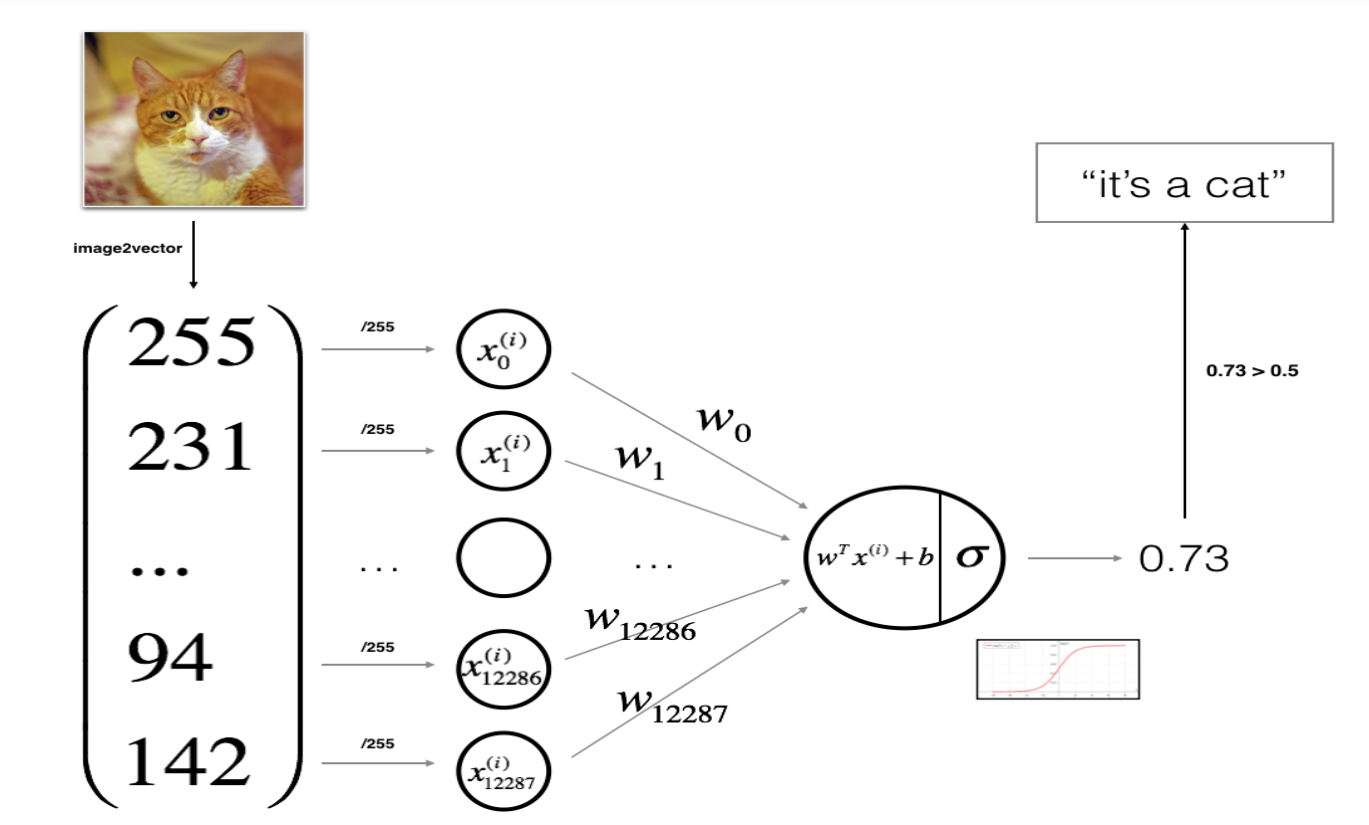
\includegraphics[scale=.5]{cat_log} \\
	Above is a depication of how our Logistic Regression Neural Network will operate (refer to the previous section for an explanation of the mathematical expressions). We will carry out the following steps: \\
	\hspace*{3mm} - Initialize the parameters of the model. \\
	\hspace*{3mm} - Learn the parameters for the model by minimizing the cost. \\
	\hspace*{3mm} - Use the learned parameters to make predictions (on the test set). \\
	\hspace*{3mm} - Analyse the results and conclude. \vspace*{2mm} \\
	Lets begin building the parts of our algorithm. There are 3 main steps for \textbf{building a Neural Network}: \\
	\hspace*{3mm} 1. Define the model structure (such as number of input features). \\
	\hspace*{3mm} 2. Initialize the model's parameters. \\
	\hspace*{3mm} 3. Loop: \\
	\hspace*{7mm} - Calculate current loss (forward propagation). \\
	\hspace*{7mm} - Calculate current gradient (backward propagation). \\
	\hspace*{7mm} - Update parameters (gradient descent). \newpage
%%%% PAGE 6 %%%%

	\begin{lstlisting}
	def sigmoid(z):
		# Compute sigmoid of z = w.T * x + b
		s = 1 / (1+np.exp(-z))
		return s
	
	def initialize_with_zeros(dim):
		# Creates a vector of zeros of shape (dim, 1) for w and initializes b=0.
		w = np.zeros((dim,1))
		b = 0
		return w, b \end{lstlisting} \vspace*{1mm} 
	Now that your parameters are initialized, you can do the \textbf{forward/backward propagation} steps for learning the parameters. The steps for forward propagation are: \vspace*{1mm} \\
	\hspace*{3mm} - You get X \\
	\hspace*{3mm} - You compute $A = \sigma(w^T X + b) = (a^{1}, a^{2}, ..., a^{m-1}, a^{m})$ \\
	\hspace*{3mm} - You calculate the cost function: $J = -\frac{1}{m}\sum_{i=1}^{m}y^{i}\log(a^{i})+(1-y^{i})\log(1-a^{i})$  \vspace*{2mm} \\
	The steps for back propagation are: \vspace*{1mm} \\
	\hspace*{3mm} - Compute $ \frac{\partial J}{\partial w} = \frac{1}{m}X(A-Y)^T$ \vspace*{1mm}\\
	\hspace*{3mm} - Compute $ \frac{\partial J}{\partial b} = \frac{1}{m} \sum_{i=1}^m (a^{i}-y^{i})$
	\begin{lstlisting}
	def propagate(w, b, X, Y):
		"""
		Implement the cost function and its gradient for the propagation explained above
		Arguments:
		w -- weights, a numpy array of size (num_px * num_px * 3, 1)
		b -- bias, a scalar
		X -- data of size (num_px * num_px * 3, number of examples)
		Y -- true "label" vector (containing 0 if non-cat, 1 if cat) of size (1, m)
		
		Return:
		cost -- negative log-likelihood cost for logistic regression
		dw -- gradient of the loss with respect to w, thus same shape as w
		db -- gradient of the loss with respect to b, thus same shape as b
		"""
		
		m = X.shape[1]
		
		# FORWARD PROPAGATION (FROM X TO COST)
		A = sigmoid(np.dot(w.T, X) + b) # compute activation
		cost = -(1/m)*np.sum(Y*np.log(A) + (1-Y)*np.log(1-A)) # compute cost
		
		# BACKWARD PROPAGATION (TO FIND GRAD)
		dw = (1/m) * np.dot(X, (A-Y).T)
		db = (1/m) * np.sum(A-Y)
		
		cost = np.squeeze(cost)
		grads = {"dw": dw,
		         "db": db}
		
		return grads, cost \end{lstlisting} \vspace*{1mm} 
	Now that we have intialized our parameters and can compute a cost function and its gradient, we can create an  \textbf{optimize function} to update the parameters using gradient descent. The goal is to learn \textit{w}  and \textit{b} by minimizing the cost function J . For a parameter $\theta$ , the update rule is $\theta = \theta - \alpha d\theta$ , where $\alpha$  is the learning rate. \vspace*{1mm} \\
	We can also create a \textbf{predict} function with our learned parameters to make predictions for a dataset X. We will calculate $\hat{Y}$ = A, and then convert entries to 0 or 1 based on probabilities. \newpage
%%%% PAGE 6 %%%%

	\begin{lstlisting}
	def optimize(w, b, X, Y, num_iterations, learning_rate, print_cost = False):
		"""
		Arguments:
		w -- weights, a numpy array of size (num_px * num_px * 3, 1)
		b -- bias, a scalar
		X -- data of shape (num_px * num_px * 3, number of examples)
		Y -- true "label" vector (containing 0 if non-cat, 1 if cat), of shape (1, m)
		num_iterations -- number of iterations of the optimization loop
		learning_rate -- learning rate of the gradient descent update rule
		print_cost -- True to print the loss every 100 steps
		
		Returns:
		params - dictionary containing the weights w and bias b
		grads - the gradients of the weights and bias with respect to the cost function
		costs - list of all the costs computed during the optimization (graphing)
		"""
		costs = []
		
		for i in range(num_iterations):
			grads, cost = propagate(w, b, X, Y)
			
			dw = grads["dw"] # Retrieve derivatives from grads
			db = grads["db"] # Retrieve derivatives from grads
			
			w = w - learning_rate * dw # update rule
			b = b - learning_rate * db # update rule
			
			if i % 100 == 0: # Record the costs
				costs.append(cost)
			
			if print_cost and i % 100 == 0: # Print the cost every 100 training iterations
				print ("Cost after iteration %i: %f" %(i, cost))
		
		params = {"w": w, "b": b}
		grads = {"dw": dw, "db": db}
		return params, grads, costs
	
	def predict(w, b, X):
	'''
	Predict whether the label is 0 or 1 using learned  parameters (w, b)
	
	Arguments:
	w -- weights, a numpy array of size (num_px * num_px * 3, 1)
	b -- bias, a scalar
	X -- data of size (num_px * num_px * 3, number of examples)
	
	Returns a numpy array (vector) containing all predictions (0/1) for the examples in X
	'''
	m = X.shape[1]
	Y_prediction = np.zeros((1,m))
	w = w.reshape(X.shape[0], 1)
	
	# Compute "A" predicting the probabilities of a cat being present in the picture
	A = sigmoid(np.dot(w.T, X) + b)
	
	for i in range(A.shape[1]): # Convert prob. A[0,i] to actual predictions p[0,i]
		Y_prediction[0,i] = A[0,i] > 0.5 
	
	assert(Y_prediction.shape == (1, m))
	
	return Y_prediction \end{lstlisting} \newpage
%%%% PAGE 8 %%%%

	\noindent The final step is to \textbf{merge all functions into a model} by putting together the previous parts in the correct order. 
	\begin{lstlisting}
	def model(X_train, Y_train, X_test, Y_test, num_iterations = 2000, 
					  learning_rate = 0.5, print_cost = False):
		"""
		Arguments:
		X_train -- training set represented by a np array (num_px * num_px * 3, m_train)
		Y_train -- training labels represented by a np array (1, m_train)
		X_test -- test set represented by a np array (num_px * num_px * 3, m_test)
		Y_test -- test labels represented by a np array (1, m_test)
		num_iterations -- hyperparameter used to optimize the parameters
		learning_rate -- hyperparameter used in the update rule of optimize()
		print_cost -- Set to true to print the cost every 100 iterations
		
		Returns:
		d -- dictionary containing information about the model.
		"""
		w, b = initialize_with_zeros(X_train.shape[0]) # initialize parameters with zeros 
		
		# Gradient descent
		parameters, grads, costs = optimize(w, b, X_train, Y_train, num_iterations, 
										                    learning_rate, print_cost)
		
		# Retrieve parameters w and b from dictionary "parameters"
		w = parameters["w"]
		b = parameters["b"]
		
		Y_prediction_test = predict(w, b, X_test) # Predict test set examples
		Y_prediction_train = predict(w, b, X_train) # Predict test set examples

		# Print train/test Errors
		print("train accuracy: {} %".format(100 - np.mean(np.abs(Y_prediction_train - 
		                                                         Y_train)) * 100))
		print("test accuracy: {} %".format(100 - np.mean(np.abs(Y_prediction_test - 
		                                                        Y_test)) * 100))
		d = {"costs": costs,
		     "Y_prediction_test": Y_prediction_test, 
		     "Y_prediction_train" : Y_prediction_train, 
		     "w" : w, 
		     "b" : b,
		     "learning_rate" : learning_rate,
		     "num_iterations": num_iterations}
		
		return d 
		
	d = model(train_set_x, train_set_y, test_set_x, test_set_y, num_iterations = 2000, 
	          learning_rate = 0.005, print_cost = True) \end{lstlisting} \vspace*{1mm}
	\begin{minipage}[c]{6cm}
	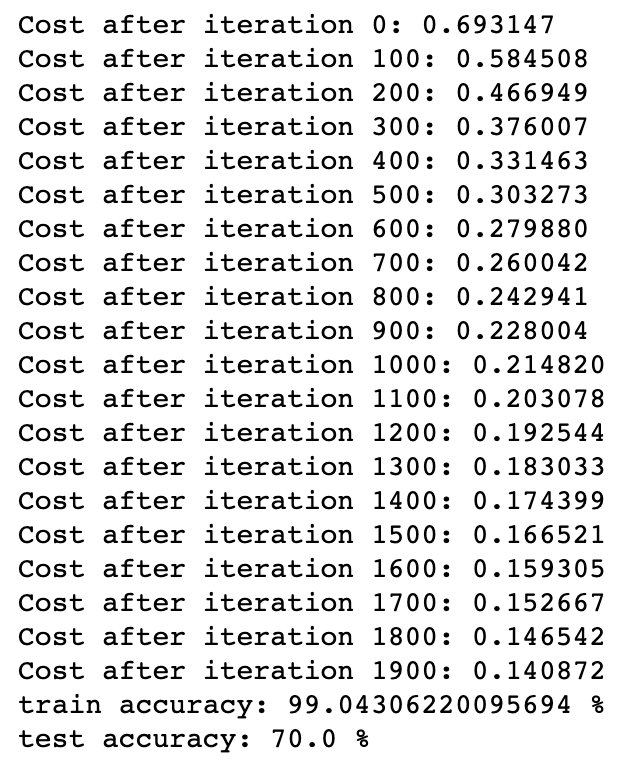
\includegraphics[scale=0.4]{model_output}
	\end{minipage}
	\begin{minipage}[c]{11cm}
	From our model, we can see that the training accuracy is 99\% while the test accuracy is 70\%, which is a cause of overfitting. We can also see that the cost is decreasing per onehundred iterations (meaning the parameters are being leaned). We can continue to idecrease the cost by increasing the number of iterations, but this will also cause more offerfitting to occur. Given the small dataset and the fact that Logistic Regression is a linear classifier, overall it is not a bad simple model. In the future, we will learn to avoid overfitting and increase the test accuracy.
	\end{minipage} \newpage
%%%% PAGE 9 %%%%

	\subsection{Shallow Neural Network}
	\subsubsection{Overview and Representation}
	Previously, we only had a single sigmoid function in our Logistic Regression model. Now, we will stack multiple sigmoids ontop of one another, followed by then feeding these into another sigmoid to create a Nerual Network. Some new notation we are introducing: \vspace*{1mm} \\
	\hspace*{3mm} - [\#] will refer to quanities associated with a given layer. \\
	\hspace*{3mm} - (i) will refer to the i$^{th}$ training example (similar to the previous section). \\
	\hspace*{3mm} - a$^{[0]}$ will be the activation layer (same as our vector x that has the input features). \\
	\hspace*{3mm} - a$^{[1]}$ will be the values for our hidden layer. \\
	\hspace*{3mm} - a$^{[2]}$ will be the output layer values (our $\hat{y}$). \\
	\hspace*{3mm} - a$^{[l]}_i$ will be [\textit{l}] = layer, \textit{i} = node in the layer. \vspace*{1mm} \\
	We will be focusing on a \textbf{Two Layer Neural Network}, which has an input layer, one hidden layer, and an output layer. We don't count the input layer as an ``official" layer. The \textit{hidden layer} will have parameters $w^{[1]}$ and $b^{[1]}$, while the output layer has parameters $w^{[2]}$ and $b^{[2]}$ associated with it. 
	\hspace*{16mm} 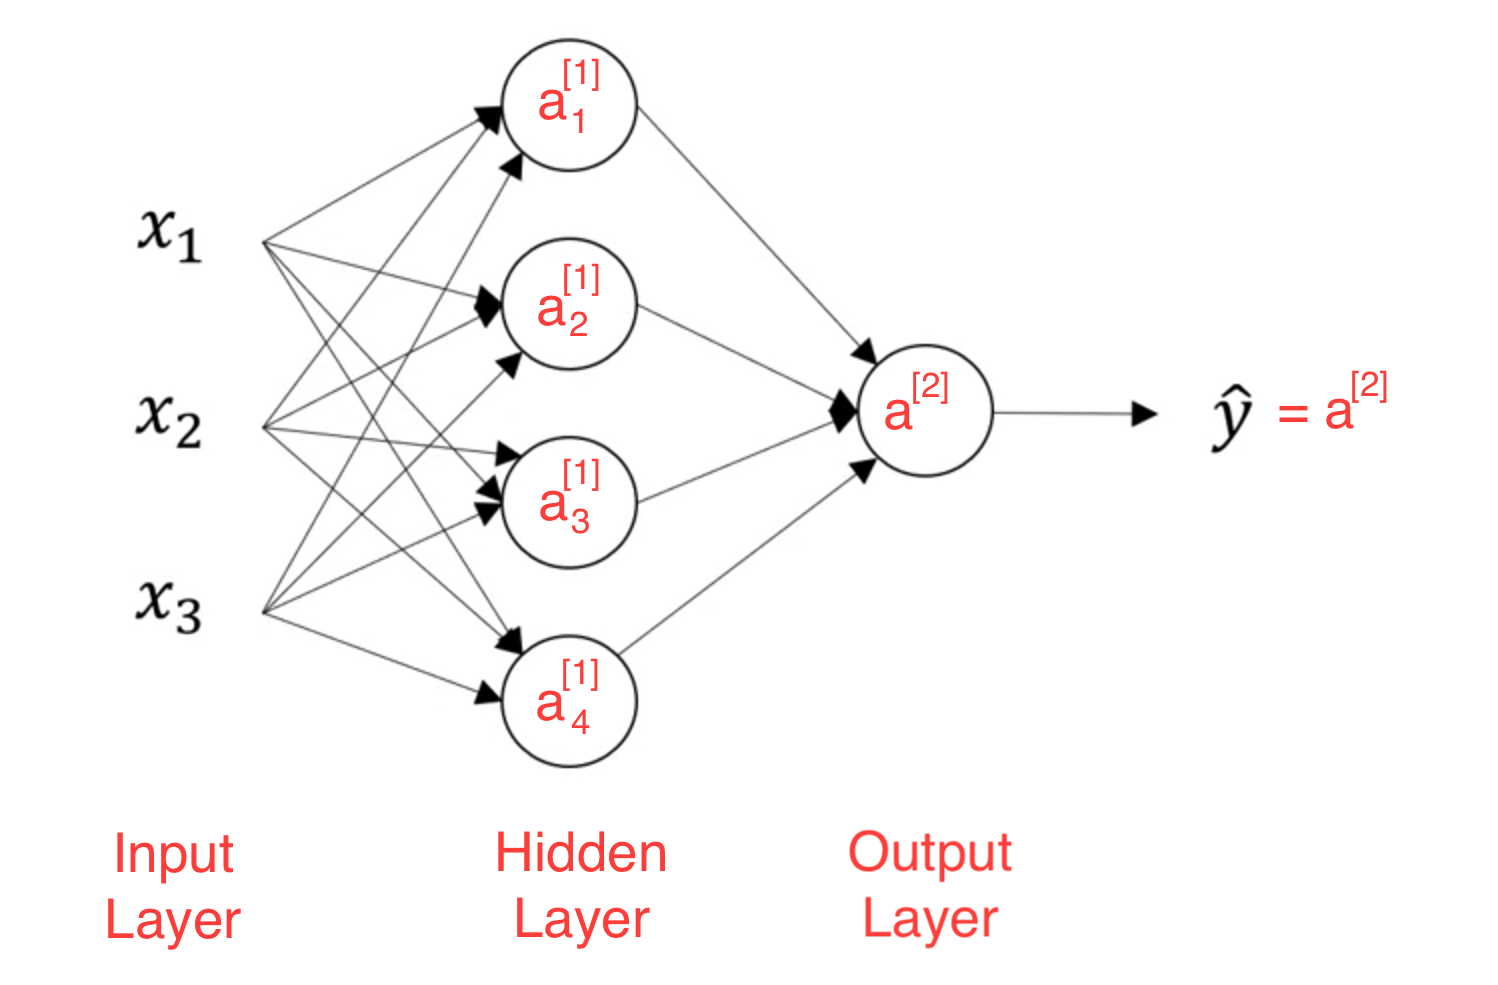
\includegraphics[scale=.5]{NN_rep} 
	\subsubsection{Computing a Neural Network Output}
	\begin{minipage}[c]{9cm}
	Each node in our hidden layer will take all of the input values from x, compute z, and input this value into an activation function (sigmoid). Since each node has to compute z, we will vectorize this process by using matrix multiplication in python. This gives us the following equation to find our vector $z^{[1]}$ and our activation vector $a^{[1]}$ for the hidden layer.
	\end{minipage}
	\begin{minipage}[c]{5cm}
	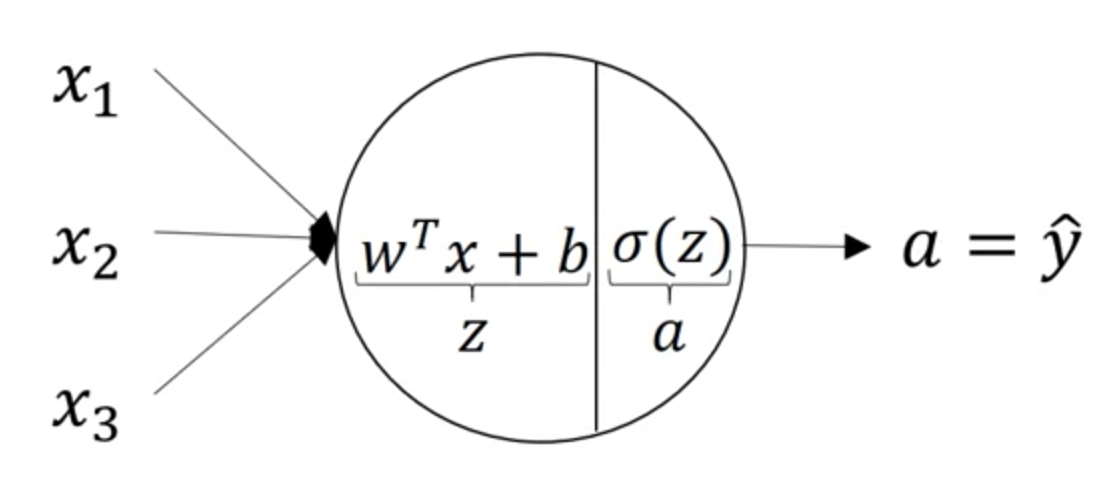
\includegraphics[scale=0.4]{act_func}
	\end{minipage} \vspace*{4mm} \\
	$$ z^{[1]} = \begin{bmatrix} -\, w_1^{[1]T}\, - \vspace*{.5mm} \\ -\, w_2^{[1]T}\, - \vspace*{.5mm} \\ -\, w_3^{[1]T}\, - \vspace*{.5mm} \\ -\, w_4^{[1]T}\, - \vspace*{.5mm} \end{bmatrix} * \begin{bmatrix} x_1 \\ x_2 \\ x_3 \end{bmatrix} + \begin{bmatrix} b_1^{[1]} \vspace*{.5mm}\\ b_2^{[1]} \vspace*{.5mm}\\ b_3^{[1]} \vspace*{.5mm}\\ b_4^{[1]} \vspace*{.5mm}\\  \end{bmatrix} = \begin{bmatrix} w_1^{[1]T}x + b_1^{[1]} \vspace*{.5mm} \\ w_2^{[1]T}x + b_2^{[1]}  \vspace*{.5mm} \\ w_3^{[1]T}x + b_3^{[1]} \vspace*{.5mm} \\ w_4^{[1]T}x + b_4^{[1]}  \vspace*{.5mm} \end{bmatrix} = \begin{bmatrix} z_1^{[1]} \vspace*{.5mm}\\ z_2^{[1]} \vspace*{.5mm}\\ z_3^{[1]} \vspace*{.5mm}\\ z_4^{[1]} \vspace*{.5mm}\\  \end{bmatrix},\;\; \text{also let}\; a^{[1]} = \begin{bmatrix} a_1^{[1]} \vspace*{.5mm}\\ a_2^{[1]} \vspace*{.5mm}\\ a_3^{[1]} \vspace*{.5mm}\\ a_4^{[1]}  \end{bmatrix} = \sigma(z^{[1]}) $$
	Note: Let the matrix with the \textit{w} values be denoted as $W^{[1]}$ and the vector holding \textit{b} values be $b^{[1]}$. \newpage
%%%% PAGE 10 %%%%

	\noindent For the \textbf{hidden layer}, this gives us the general formulas (remember x = $a^{[0]}$): \vspace*{1mm} \\
	\hspace*{3mm} $z^{[1]} = W^{[1]}a^{[0]} + b^{[1]}$ with shapes: $z^{[1]}=(4,1),\; W^{[1]}=(4,3),\; a^{[0]}=(3,1),\; b^{[1]}=(4,1)$ \vspace*{1mm} \\
	\hspace*{3mm} $a^{[1]} = \sigma(z^{[1]})$ with shapes: $a^{[1]}=(4,1),\; z^{[1]}=(4,1)$ \vspace*{2mm} \\
	For the \textbf{output layer}, this gives us the following formulas (ouput $a^{[1]}$ used as input ``x"): \vspace*{1mm} \\
	\hspace*{3mm} $z^{[2]} = W^{[2]}a^{[1]} + b^{[2]}$ with shapes: $z^{[2]}=(1,1),\; W^{[2]}=(1,4),\; a^{[1]}=(4,1),\; b^{[2]}=(1,1)$ \vspace*{1mm} \\
	\hspace*{3mm} $a^{[2]} = \sigma(z^{[2]})$ with shapes: $a^{[2]}=(1,1),\; z^{[2]}=(1,1)$
	\subsubsection{Vectorizing Across Multiple Examples}
	When we want to compute predictions for all of our training examples (not just a single example like we did above), we need to vectorize a method in order to compute all of these at once. Some new notation we will use: \vspace*{1mm} \\
	\hspace*{3mm} - ex: a$^{[2](i)}$ refers to the layer 2 value for the i$^{th}$ training example. \vspace*{1mm} \\
	We will define the following matrices to work with $n_x$ training examples where X = m training examples, Z$^{[1]}$ = is all of the z$^{[1]}$ values for m training example, and A$^{[1]}$ = all of our a$^{[1]}$ values for m training examples. Note that the format is the same for Z$^{[2]}$ and A$^{[2]}$ with their corresponding values. $$ X = \begin{bmatrix} | & | & ... & | \\ x^1 & x^2 & ... & x^m \\ | & | & ... & | \end{bmatrix} \hspace*{5mm} Z^{[1]} = \begin{bmatrix} | & | & ... & | \\ z^{[1](1)} & z^{[1](2)}  & ... & z^{[1](m)}  \\ | & | & ... & | \end{bmatrix} \hspace*{5mm} A^{[1]} = \begin{bmatrix} | & | & ... & | \\ a^{[1](1)} & a^{[1](2)}  & ... & a^{[1](m)}  \\ | & | & ... & | \end{bmatrix} $$
	This gives us the following \textbf{vectorized formulas} to find all predicted values for m examples: \vspace*{1mm} \\
	\hspace*{3mm} $Z^{[1]} = W^{[1]}X + b^{[1]}$  \vspace*{1mm} \\
	\hspace*{3mm} $A^{[1]} = \sigma(Z^{[1]})$  \vspace*{1mm} \\
	\hspace*{3mm} $Z^{[2]} = W^{[2]}A^{[1]} + b^{[2]}$  \vspace*{1mm} \\
	\hspace*{3mm} $A^{[2]} = \sigma(Z^{[2]})$ \vspace*{2mm} \\
	
	
	
	
	
	
\end{spacing}
\end{document}